% !TeX root = ../main.tex

\chapter{Device evaluation and dispersion analysis of samples fabricated using various CVD methods}\label{chap:5}% from transmission spectroscopy
During and after the fabrication, the film property and devices are then fully estimated. To compare the chemical vapor deposition method differences, the material properties, especially the infrared band absorption is first studied. By using tunable laser based spectrum measurement, device optical transmission is then analyzed. Finally, this chapter is closed by the discussion of dispersion behavior shown in fabricated devices.

\section{Material properties}

\subsection{Ellipsometry}

%It is more necessary to evaluated the refractive indexes of the film deposited above. 
Using the infrared ellipsometry, the refractive index of deposited silicon nitride film is obtained. The result is shown in \autoref{fig:ellipso}, where we can see the index varies from the deposition methods at the magnitude of 0.01. 
Furthermore, even the refractive index are distinguished, the material wavelength dispersion parameter $D_M$ can be close.

\subsection{Fourier-transform infrared spectroscopy}

The vast majority of studies on silicon nitride fabrication processes have found that the hydrogen remaining in the films leads to N-H and Si-H bonds, which causes the optical absorption at S and C band \cites{Ay2004, Agnihotri2000}. To quantitatively clarify these bonds in our film, we perform the Fourier-transform infrared spectroscopy (FTIR) on the top of silicon nitride film.

The measurement is carried out using attenuated total reflection (ATR) method with SHIMADZU IRTracer-100. In \autoref{fig:ftir}, the absorbance is taken from the difference with background transmittance. It can be seen that except the peak around 780 \si{\per\cm} referring to Si-N stretching mode, two other peaks are located around 2150 \si{\per\cm} and 3350 \si{\per\cm}, corresponding to Si-H and N-H bonds respectively.

Interestingly, there are also two peaks found at 1020 \si{\per\cm} and 1120 \si{\per\cm}, indicating Si-O symmetric and asymmetric stretching modes in bottom silica. This result may be explained by the fact that in ATR method, the depth of penetration at this wavelength is less than 1 micron, while the thickness of silicon nitride layers in our experiment is targeted at 800 nm.
% \cite{Shaw2005}


\begin{figure}
	\centering
	\includesvg[width=.6\textwidth]{ftir}
	\mycaption{Absorbance of deposited film using Fourier-transform infrared spectroscopy}{S-H and N-H bonds are obvious in LS-CVD and PE-CVD films.}
	\label{fig:ftir}
\end{figure}

In conclusion, even though the ammonia free recipe is used in LS-CVD method, the film is still hydrogenated while LP-CVD commercial wafers show least N-H absorbance.

\begin{figure}
	\centering
	\includesvg[scale=0.7]{ellipso}
	\mycaption{Refractive index and evaluated material dispersion of the film deposited measured via ellipsometry}{The dispersion parameter is calculated by second-order difference of fitted Sellmeier equations.}
	\label{fig:ellipso}
\end{figure}

\section{Device transmission}

\subsection{Methods}

In the example given in \autoref{sec:disp-comp},  a typical dispersive ring resonator has the $ D_2 $ value around MHz, which means the given free spectra range (FSR), for example 100 GHz, is greater than the next one in a MHz-level difference. It is difficult to achieve such precise measurement using traditional optical spectrum analyzer whose typical resolution is around pm, 100 MHz. The tunable laser scanning is developed to solve this problem, especially assisted by an external frequency comb \cite{Liu2016d}. 

Here, we exploit the method using laser step triggering to calibrate the real-time measured device transmission. Compared with the frequency comb or wave meter assisted spectroscopy, this method is much more convenient to deploy. By increasing the data acquisition sampling rate or alternating with electric oscilloscope, the wavelength precision can be further improved.
Given the well-resonant spectrum, the dispersion information is further extracted from the transmission, in particular the resonant peaks. 
%Such method is widely used to study the Kerr frequency comb. It is also efficient to study the frequency-entangled photon pair generation.

\begin{figure}
	\centering
	\includesvg[scale=1]{align}
	\mycaption{Images of fiber launching setup}{\textbf{a} A lensed fiber is aligned to the end of bus waveguide. \textbf{b} Chip carried over a thermoelectric cooler. \textbf{c} Photo of waveguide end taken using infrared camera. \textbf{d} Optical microscope of fabricated sample.}
	\label{fig:align}
\end{figure}

\subsubsection{Fiber launching} 

Using two five-axis fiber alignment stages (Newport M-562F-XYZ \& M-562F-XYZ-LH), the device ports are aligned with two lensed fibers on both sides. The spot size of lensed fibers is 2 \um, see \autoref{fig:align}(a) and (b), which is not optimized to the size mentioned in \autoref{sec:edge}. 

Before any following experiments, the output port is first coupled to the infrared InGaAs camera in free space using a 20$\times$ objective lens. To align the chip input port precisely, the real-time images is used to adjust all the three degrees of freedom until the spot is observed explicitly on the screen, see \autoref{fig:align}(c). Next, by carefully rotating the palettes of polarization controller on the input side, the device coupling can be built in either TE or TM mode. Then another lensed fiber is launched instead and aligned carefully, as the power meter reading is referred to.

In this method, the best facet-to-facet coupling efficiency is around 6 dB in the case of LIGENTEC samples introduced in \autoref{chap:6}, where is optimized by mode convertors. Comparatively, a more typical facet-to-facet loss without mode convertors can be 8-9 dB.

%LS-CVD samples
It is worth mentioning that all the chips are set over a chip carrier (SURUGA SEIKI F126) equipped with a thermoelectric cooler (TEC). This is essential for long-time thermal stability, see \autoref{fig:align}(a).
With TEC connected to an external temperature controller, the temperature precision around device under test can be 0.1 \si{\celsius}.
To avoid moisture condensation, the TEC is set a little higher than room temperature, 30 \si{\celsius} in our case. 

\subsubsection{Spectrum sweeping}

\begin{figure}
	\centering
	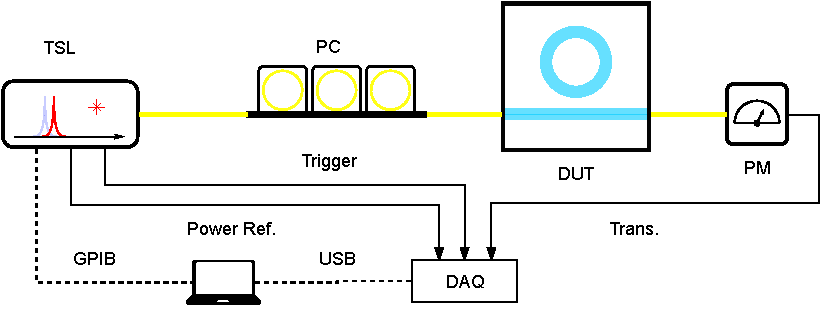
\includegraphics[width=1\textwidth]{imgs/trans.pdf}
	\mycaption{Setup of transmission measurement system}{TSL, tunable semiconductor laser. PC, optical fiber polarization controller. DUT, device under test. PM, power meter. DAQ, data acquisition.}
	\label{fig:transsetup}
\end{figure}

The schematic diagram of the device spectrum measurement is shown in \autoref{fig:transsetup}. 
After manual alignment, the tunable semiconductor laser (SANTEC TSL-710) is first set to continuously sweep from 1480 nm - 1640 nm, covering the optical communication S C and L bands.
The internal power reference signal and the step trigger are also generated simultaneously, which are used to calibrate the output optical power and improve wavelength scanning accuracy. The output power from device under test is measured by the power meter (Newport 2963-R). 

Compared with photon diodes, the power meter in our setup is critical to realize various range scanning.  Finally, the signals of power reference, step trigger and device transmission are all synchronized with the data acquisition module, and then analyzed by the computer. To achieve pm-resolution spectra, transmitted power is simply divided by power reference and the step trigger are marked to interpolate wavelengths in the certain time interval.

\subsubsection{Peak searching}

Given the transmission spectra, the negative peaks are located with peak-finding algorithm, yielding not only the peak location, but also the width and prominence. These values are next used to calculate the free spectral ranges and \textit{Q}-factors. In general, due to the fabrication difference, not all the devices appear resonance in the measured band. To compensate the broken spectra, several algorithm are performed to achieve best performance of peak-finding. 

\begin{figure}
	\centering
	\includesvg[width=4in]{filt_cf}
	\mycaption{Illustration of peaking searching}{The digital filter is used to process the raw transmission for better performance of peak searching algorithm.}
	\label{fig:spec_filt}
\end{figure}

In our technology, for the spectra with remarkable absorption illustrated in \autoref{fig:spec_filt}, the background of raw spectrum is first calculated using digital filters. The filtered spectra are then used to search the peaks without the noise effects.


\subsection{Thermal stability}

\begin{figure}
	\centering
	\includesvg[width=1\textwidth]{thermal_depen}
	%	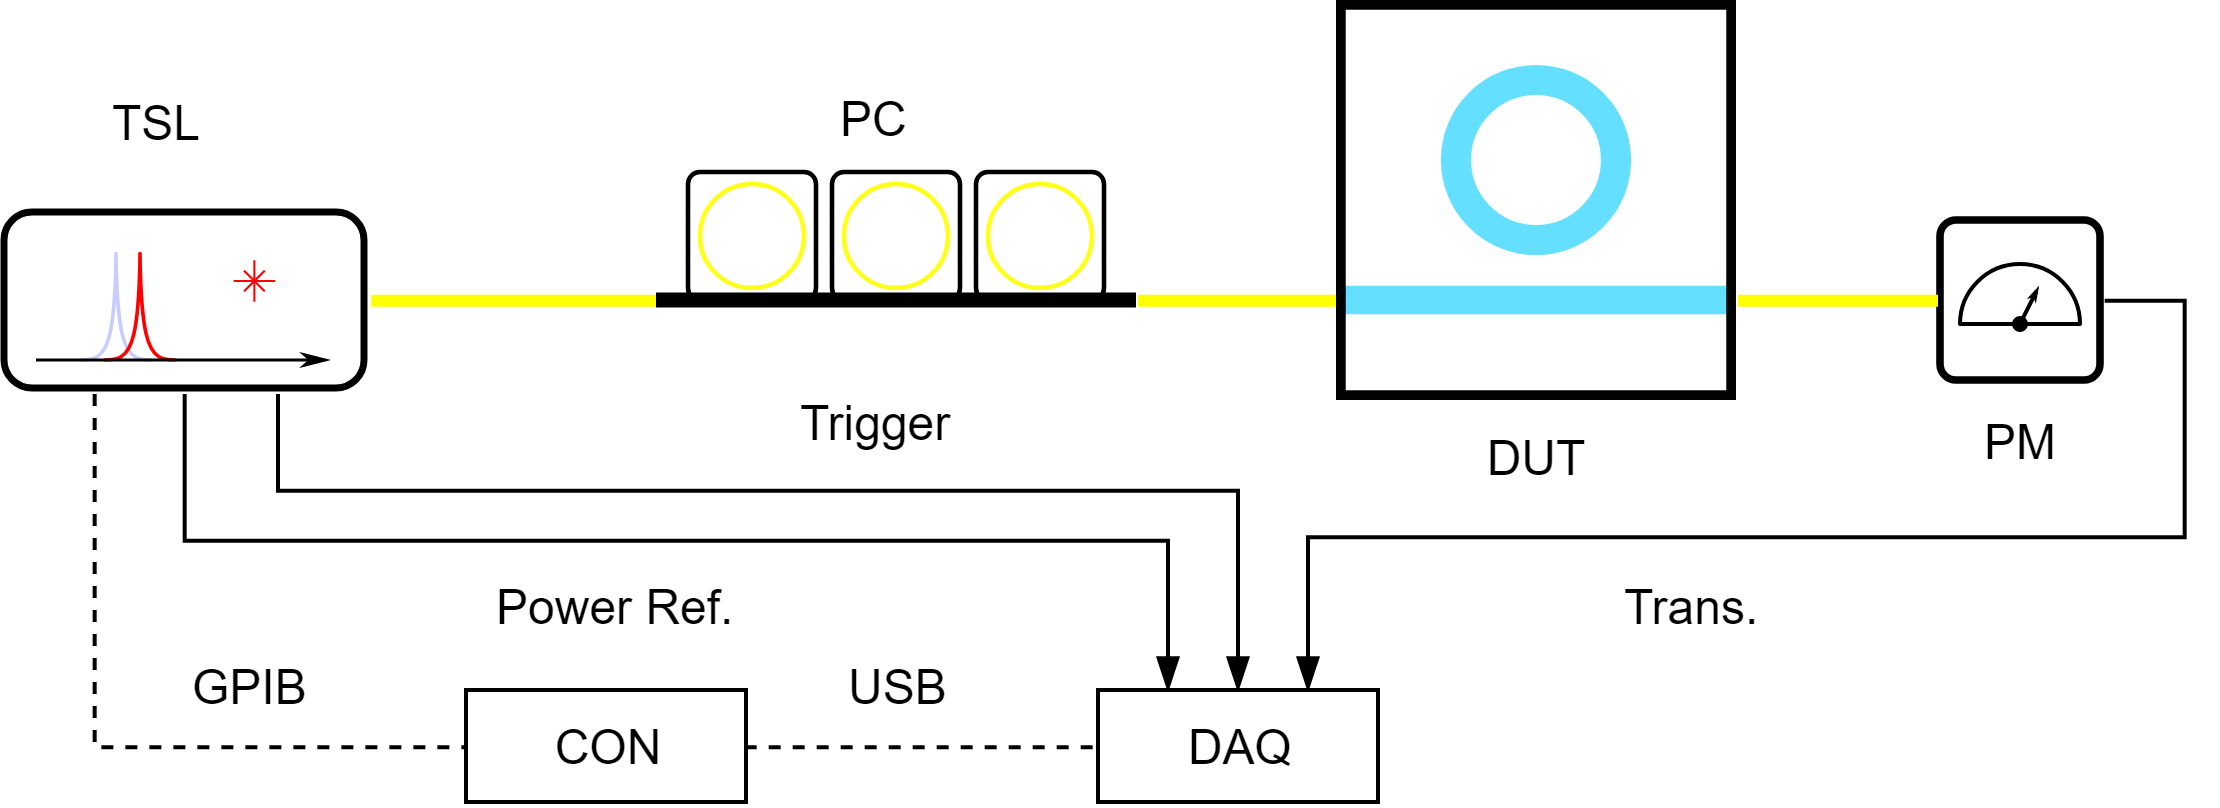
\includegraphics[width=.9\textwidth]{imgs/png/trans_setup}
	\mycaption{Thermal dependence of LP-CVD sample}{\textbf{a}. Transmission measured at three temperatures. \textbf{b}. Resonant wavelengths extracted versus temperature. The estimated thermal dependence $\dv*{\lambda}{T}$ is 23 \si{\nm/\celsius}.}
	\label{fig:thermal}
\end{figure}

Although silicon nitride is reported as high thermal conductivity material, the surrounding silicon dioxide is comparatively worse thermal conductive. Despite the room temperature fluctuation, the nonlinear phenomena usually requires high pump power intracavity, which heats the device significantly. In result, refractive index occurs and leads to resonance shift. Thus, the thermal sensitivity is a critical factor of nonlinear ring resonators.

For example, with the TEC set into different temperatures, the spectrum of same LP-CVD sample is then measured. Shown in \autoref{fig:thermal}(a), temperature increasing leads to a obvious red-shift of the resonant peak. The wavelength range around 1630 nm is chosen for better transmission in this device. From \autoref{fig:thermal}(b), the estimated thermal dependence of resonant wavelength $\dv*{\lambda}{T}$ is 23 \si{\nm/\celsius}. In this case, if the \textit{Q}-factor of ring resonator is up to \num{d5}, even room temperature variation can results in totally off-resonance.

\subsection{Results}

To compare the material difference among the films deposited in three CVD methods, identical ring resonators layout is targeted to fabricate all these samples, film thickness is 800 nm, ring width is 1.5 \um and ring radius is 200 \um. %Controlling thickness 
Since the thickness control during the film deposition and ICP etching is tough, all the devices are label with the waveguide height measured by step profiler before TEOS top cladding. In particular, LP-CVD device is 802 nm-thick and LS-CVD device is 885 nm-thick.

However, the fabrication of stoichiomertric silicon nitride using PE-CVD 
\\method is not successful, a sample deposited using same machine but with a silicon-rich recipe is reported instead. 

The device transmission spectrum is first measured, shown in \autoref{fig:cvd_cf}(a). It can be seen that there is strong optical absorption from 1500 nm to 1540 nm in each device. 
Recording to the FTIR result shown in \autoref{fig:ftir}, in particular LP-CVD sample containing almost no Si-H or N-H bonds, 
the optical absorption may originate from not only the residual hydrogen in silicon nitride but also top-cladding or bottom buried TEOS layer. 

In addition, LP-CVD sample shows absorption at some certain wavelength, leading to the error values of peak finding. Such kind of broken spectra can be probably explained by the fabrication toleration, such like the gap is not fully etched or the ring resonator is contaminated. All these fabrication imperfection plays the role of scattering and also decreases the quality factors.

Furthermore, from the extracted resonant peaks, the \textit{Q}-factors and frequency FSRs are summarized in \autoref{fig:cvd_cf}(b). The radius of each ring resonator are designed as 200 \um, corresponding to the FSR of 119.3 GHz. This agrees with the extracted FSRs of LP-CVD and LS-CVD devices. In the case of silicon-rich PE-CVD sample, the measured FSR of ring resonators near 1550 nm is around 94.3 GHz, indicating the refracting index of silicon-rich silicon nitride film is 0.34 higher.

In the term of \textit{Q}-factors, counted in \autoref{fig:cvd_cf}(c), the LS-CVD samples have the highest quality factors whose mean value is \num{2.7d4} whereas the one of silicon-rich PE-CVD samples is \num{1.8e4}. The \textit{Q} factor trend of LP-CVD device are similar to LS-CVD ones, but influenced by the broken resonance spectrum.

\begin{figure}[t]
	\centering
	\includesvg[height=6in]{cvd_cf}
	\mycaption{Comparison of device transmission, quality factors and FSR between three CVD methods}{Identical ring resonators layout is used to fabricate all these samples, film thickness is 800 nm, ring width is 1.5 \um and ring radius is 200 \um.}
	\label{fig:cvd_cf}
\end{figure}


%Beyond the samples with same design, LS-CVD deposited and sputtering films also succeed to 
%...


\section{Dispersion analysis}

Previous work \cite{Sunada2018} gave two methods analyzing the device dispersion, both depending on device transmission. One is to perform Fourier transform of the reflected spectra on the input port, which is equivalent to an etalon interference whose mirrors are waveguide input and output facets. Another method employs the cavity resonance instead. Despite the fabrication tolerance, considering the bent segment, the chromatic dispersion in the ring resonator is not identical to the one in straight waveguides. Hence in our research, to the extract dispersion information accurately, the ring resonance method is preferred. 

Following the integrated dispersion definition, the resonant wavelength $\lambda_m$ is first converted to resonant frequencies $\omega_m$. Before the polynomial fitting, the linear fitting is performed to evaluate first-order mode dispersion parameter. Then the integrated dispersion is calculated using the formula $ \dint(\mu) = \omega_0 - D_1 \mu$. The central frequency is $\omega_0$ set as the center of scanning range. The relative mode numbers are constructed as a integer neighborhood of zero. A final step is the cubic or quadratic polynomial fitting. For a wider range scanning, a quartic curvature is more efficient, but in our case, the cubic polynomial is sufficient to extract second-order dispersion parameters in a 160 nm span.

For the samples fabricated using subtractive processes, due to the fabrication imperfection, not all the devices show efficient resonance, especially for LP-CVD and PE-CVD. The dispersion of devices fabricated above is only analyzed in the non-absorption range, 1550 - 1560 nm, shown in \autoref{fig:dint_cvd_cf}. As we can see, in the case of LP-CVD and PE-CVD deposited films, thanks to the fine control of waevguide dimension, the dispersion are efficiently compensated. While due to different recipe used in PE-CVD one, non-stoichiomertric silicon nitride stands out lagers material dispersion.

\begin{figure}
	\centering
	\includesvg[width=4in]{cvd_dint_cf}
	\mycaption{Integrated dispersion of devices fabricated using different CVD methods}{Evaluated second-order dispersion of LP-CVD and LS-CVD devices presents near perfect dispersion compensation.}
	\label{fig:dint_cvd_cf}
\end{figure}


\section{Summary}

From the above result, the high \textit{Q}-factor up to \num{5d4} is achieved using subtractive process though, in extensive experiments, no frequency conversion succeeded even with 100 mW level pump power. A possible explanation is that residual hydrogen in the CVD deposited films not only leads to near infrared range absorption, but also changes the effective nonlinear interaction of Si-N bonds. In this perspective, annealing processes is urgently demanded in our current fabrication flow.